
\paragraph{1. Preserving \textit{happens-before} relations}
        
    If $\stck{_{hb}}$ relations among events are lost after reordering, they may introduce new observable behaviors. The relations that are subject to change can be divided into four parts using events $e$ and $d$.
    \begin{tasks}(2)
        \task $\reln{k}{hb}{e}$.
        \task $\reln{e}{hb}{k}$.
        \task $\reln{d}{hb}{k}$.
        \task $\reln{k}{hb}{d}$.
    \end{tasks}

    Firstly, note that the relations of the form $\reln{e}{hb}{k}$ come through either a $\stck{_{sw}}$ relation with $e$ or relations through event $d$, i.e. of the form $\reln{d}{hb}{k}$. 
    The ones that come due to the latter, may not be preserved after reordering. 
    Note also that, a similar argument exists for relations of the form $\reln{k}{hb}{d}$ wherein relations derived through $e$($\reln{k}{hb}{e}$) may be lost after reordering. 

    Hence, the relations that could be subject to change can be addressed by considering two disjoint sets of events in any \textit{Candidate Execution} of $C$ as below.
    \begin{align*}
       K_e = \{k \ | \ \reln{k}{hb}{e} \}. \\
       K_d = \{k \ | \ \reln{d}{hb}{k} \}. 
    \end{align*}

    Figure~\ref{reord:preserve_hb(a)} below pictorially shows this.
    \begin{figure}[H]
        \centering
        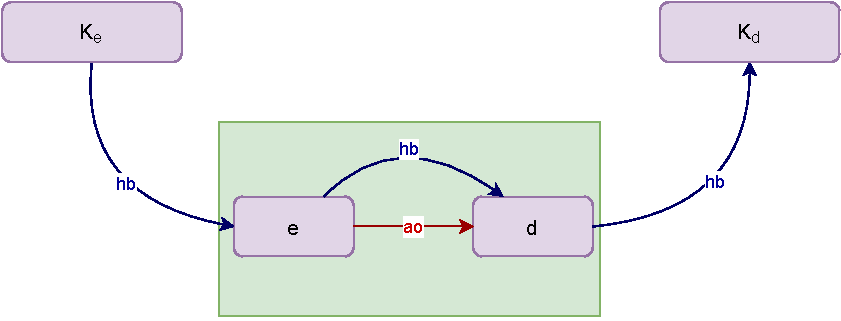
\includegraphics[scale=0.7]{5.InstructionReordering/4.ValidReorderingCandidate/ProofParts/Part1/part1(a).pdf}
        \caption{For any Candidate Execution of $C$, the set $K_e$ and $K_d$ and its relation with events $e,d$.}
        \label{reord:preserve_hb(a)}
    \end{figure}
    
    Consider two events $\event{p1}{K_e}$ and $\event{p2}{K_d}$ (When $e$ is the first event or $d$ is the last event, assume dummy events that can act as $p1$ or $p2$.) belonging to the same agent as that of $e$ and $d$ such that in $C$:
    \begin{align*}
        dir(p1,e)\ \wedge\ dir(d,p2).
    \end{align*}
    
    Note that in terms of direct happens-before relations, on reordering, any $Candidate Execution$ of $C$ will have the following changes shown in Figure~\ref{reord:preserve_hb(b)}
    \begin{figure}[H]
        \centering
        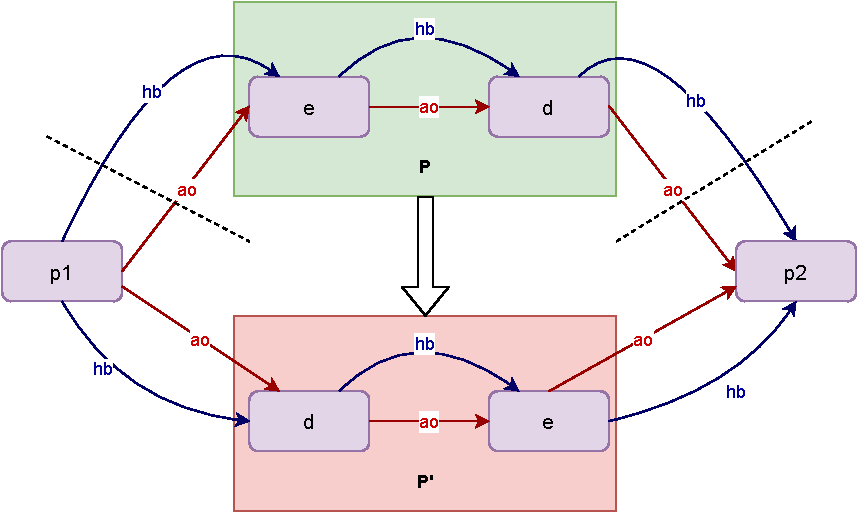
\includegraphics[scale=0.7]{5.InstructionReordering/4.ValidReorderingCandidate/ProofParts/Part1/part1(b).pdf}
        \caption{The \textit{direct happens-before} relation that change while reordering events $e$ and $d$.}
        \label{reord:preserve_hb(b)}
    \end{figure}
    
    The figure above is to show that, for any $Candidate Execution$ of $C$, the following is true
    \[
        cons(p1,e) \ \wedge dir(p1,e) \ \wedge dir(e,d) \ \wedge cons(d,p2) \ \wedge \ dir(d,p2).
    \]
    and for that of $C'$,
    \[
        cons(p1,d) \ \wedge \ dir(p1,d) \ \wedge \ dir(d,e) \ \wedge cons(e,p2) \ \wedge dir(e,p2).
    \]
    
    We need the following key relations to be preserved in Candidate executions of $C'$ 
    \begin{tasks}(2)
        \task $\reln{p1}{hb}{e}.$
        \task $\reln{e}{hb}{k}.$
        \task $\reln{d}{hb}{p2}.$
        \task $\reln{k}{hb}{d}.$ 
    \end{tasks}

    After reordering, we have (a) and (c) preserved due to transitivity  
    \begin{gather*}
        \reln{p1}{hb}{d} \ \wedge \ \reln{d}{hb}{e} \ \Rightarrow \ \reln{p1}{hb}{e}. \\
        \reln{e}{hb}{p2} \ \wedge \ \reln{d}{hb}{e} \ \Rightarrow \ \reln{d}{hb}{p2}. \\
        \reln{p1}{hb}{d} \ \wedge \ \reln{d}{hb}{e} \ \wedge \ \reln{e}{hb}{p2} \ \Rightarrow \ \reln{p1}{hb}{p2}. 
    \end{gather*}

    (b) and (d) may not be preserved due to $\reln{d}{sw}{k}$ or $\reln{k}{sw}{d}$. If we can "pivot" the  set $K_e$ to $p1$ and $K_d$ to $p2$, it would ensure that our other two intended relations also remain preserved after reordering by transitivity. To state formally, we have a valid pair of pivots $<p1,p2>$ when the following two conditions hold
    \begin{gather*}
        \forall \ k \in K_e - \{p1\}, \ \reln{k}{hb}{p1}. \\
        \forall \ k \in K_d - \{p2\}, \ \reln{p2}{hb}{k}.
    \end{gather*}
    
    By Lemma \ref{Lemma1} and \ref{Lemma2} respectively, we have for $C$, the following condition where $<p1, p2>$ is a valid pivot pair.
    \begin{gather*}
        \et{e}{uo} \vee (\et{e}{sc} \wedge \event{e}{W}). \\
        \et{d}{uo} \vee (\et{d}{sc} \wedge \event{d}{R}).
    \end{gather*}
        
    Figure~\ref{reord:preserve_hb_table} summarizes the cases where we have a valid pair of pivots\footnotemark $<p1,p2>$.
    \begin{figure}[H]
        \centering
        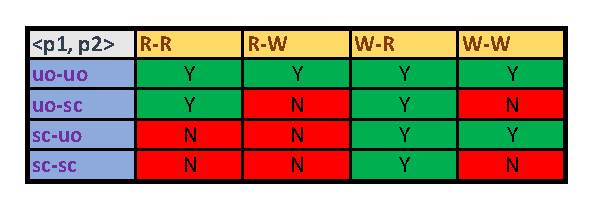
\includegraphics[scale=0.7]{5.InstructionReordering/4.ValidReorderingCandidate/ProofParts/Part1/part1_table.pdf}
        \caption{Table summarizing whether we have valid pair of pivots based on  $e$ and $d$.}
        \label{reord:preserve_hb_table}
    \end{figure}
            
    We show a simple example (Figure~\ref{reord:preserve_hb(c)} and \ref{reord:preserve_hb(d)}) where we do not have a valid pair of pivots, particularly because $p1$ is not a valid pivot. 
    Note that in this example, $K_e = K_{e1} + K_{e2} + p1 + p_x$
    \begin{figure}[H]
        \centering
        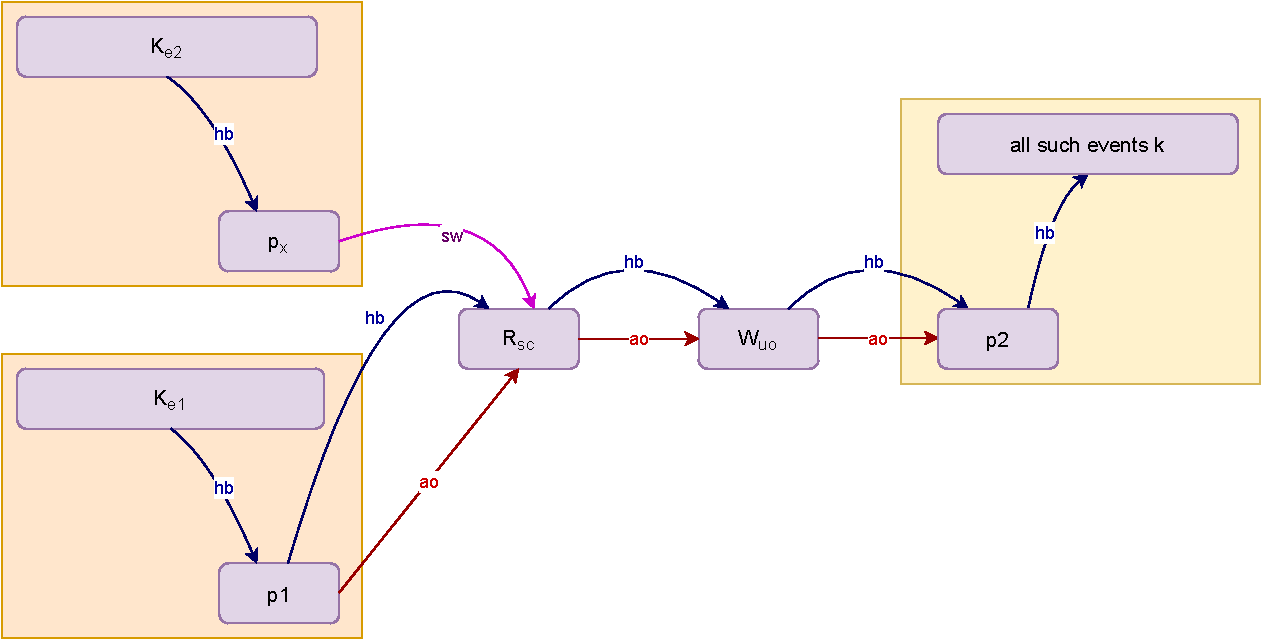
\includegraphics[scale=0.6]{5.InstructionReordering/4.ValidReorderingCandidate/ProofParts/Part1/part1(e).pdf}
        \caption{A Candidate Execution where p1 is not a valid pivot.}
        \label{reord:preserve_hb(c)}
    \end{figure}
    
    %Show figure here of program P'
    \begin{figure}[H]
        \centering
        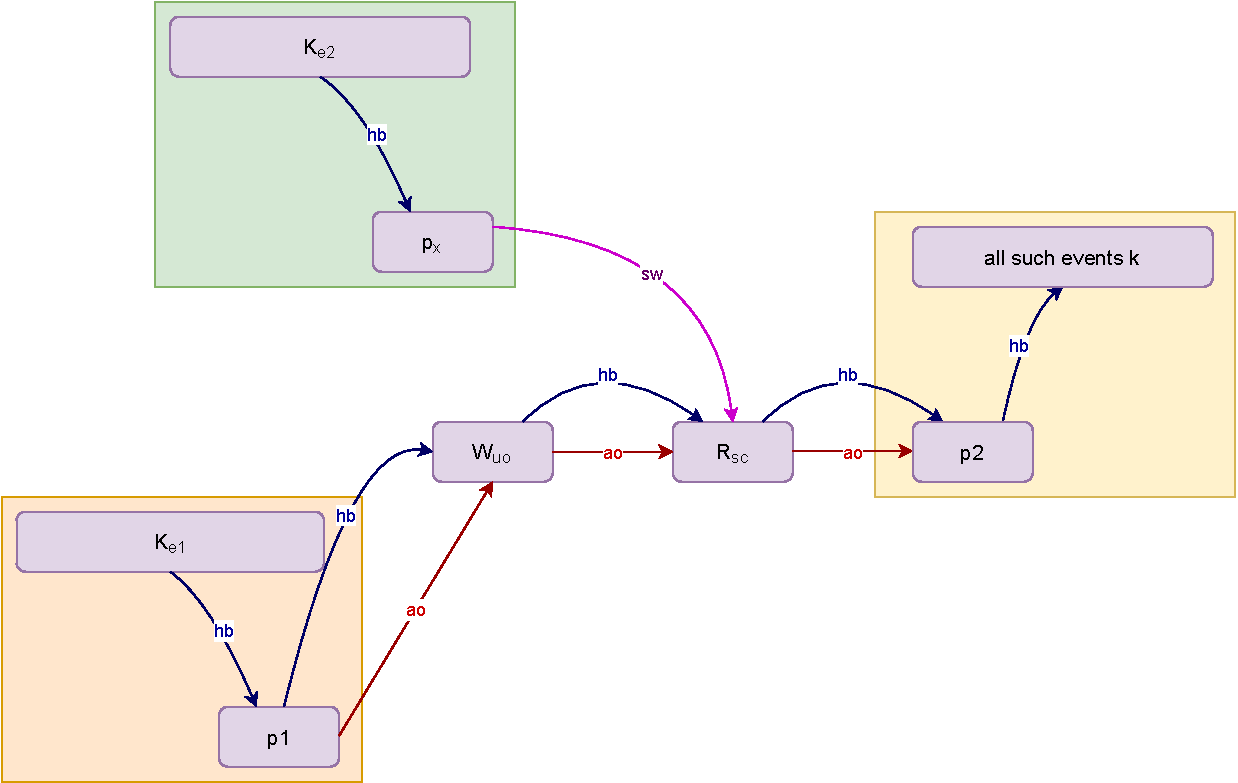
\includegraphics[scale=0.6]{5.InstructionReordering/4.ValidReorderingCandidate/ProofParts/Part1/part1(f).pdf}
        \caption{The resultant Candidate Execution after reordering, exposing the relations with $p_x$, $K_{e2}$ and $d$ that are lost}
        \label{reord:preserve_hb(d)}
    \end{figure}
        
    \footnotetext{This proof does not go about showing the exact happens-before relations that are preserved; rather it uses the properties between different happens before relations that hold, which would imply that for any possible Candidate Execution after reordering, the set of happens-before relations apart from that between $e$ and $d$ remain the same.}